\subsection{Application Flow}
As seen in figure 4.1, when starting the application a splash screen will appear because it needs to load the used NLP libraries, which will take a bit of time for it to load up. When the NLP libraries has been loaded a new window will pop up, this will be the login window where users have the ability to log in with either your admin login or the regular teacher/student login. After logging in, the chat window will appear. 
If the user has the teacher role, the person will be able to open the help request window. If the user has an administrative role, the user will both have access to the help request and the admin controls, where one can see, edit and add users, classes and materials.
\newline\newline
Each part of the application will be further explained in the next sections.

\begin{figure}[H]
    \centering
    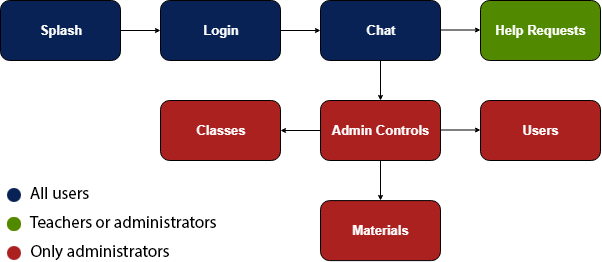
\includegraphics[width=0.65\textwidth]{figures/Flow.png}
    \caption{Application Flow}
    \label{fig:flow_chart}
\end{figure}
